\documentclass{report}
\usepackage[pdftex]{graphicx}
\usepackage[english]{babel}
\usepackage{float}
\begin{document}
\title{Temperature Monitoring System}
\author{Mike Guzior, Jason Pearson, Marcel Englmaier and Justin Koehler}
\maketitle
\tableofcontents
\newpage
\subsection*{Abstract}
\addcontentsline{toc}{subsection}{Abstract}
The goal of this project is to create an easy to use and low cost temperature monitoring system for anyone to use. 
The web end will allow the user to login in and view room statistics, as well as set warnings on thresholds. 
With the thresholds we would allow the user to select actions based on the threshold such as sending a text when it reaches a certain temperature. 
The room will contain a Raspberry Pi equipped with sensors which will use Ethernet to communicate to the web end and update information. 
The reason for using the Raspberry Pi’s is that we would be able to create a low cost sensor and be able to customize the code on the Pi as well. 
\newpage
\subsection*{Background}
\addcontentsline{toc}{subsection}{Background}
Our client has many needs that have been unmet for various reasons, with problems in their current situation, and our project provides solutions to those needs and provides resolutions to their problems.
\newline
\indent
Per Wikipedia, Western Michigan University's (WMU for short) Parkview campus was built in 2003 at a cost of $\$$72.5 million and is the home of the Western Michigan University College of Engineering and Applied Sciences (CEAS for short). 
 WMU’s engineering website explains that WMU has “state-of-the-art resources housed in a $\$$100 million high-tech facility”. 
Sadly, our client has advised that this did not include any automated temperature or humidity sensors and reporting equipment in any of the rooms. 
 These are absolutely critical in rooms that maintain computer, technology, manufacturing, and scientific equipment to safeguard the investment and resources of the university.  There are many risks that computer equipment face as the spent their entire life conducting electricity and being made of rust-prone metals. Standard servers are recommended to be kept at an average temperature of 22°C or less, with automatic shut-off or critical shutdown temperature maximums of 35°C. They must also be kept dry as any condensate will not only short any circuit boards it touches, but cause the servers themselves to rust, as well as the metal racks that support them. Aside from rusts and shorts, excess humidity is a cause of molding and mildewing which is unhealthy for personnel and students, and also damages hardware and clogs air filters. There are many factors that provoke the need for this monitoring, from the downtime of a website, to the security networks that safeguard a campus, the need to have digital phones online, to safeguard data that would be lost in a failure, to the overall cost of the hardware. As an example, one server cluster with the moniker "Thor" has a hardware value of $400,000 which would result in an excessive loss for the university if it were damaged. 
 Our client informed us that there have been several incidences where the temperature of servers increased unhindered to the point that equipment was destroyed due to this lack of automated environment reporting. One such incident where the temperature increased without staff knowing resulted in a ~$500,000 loss. A previous loss due to humidity occurred when the humidity rose to the point of condensation and large steel papermaking rolls generated a layer of surface rust, rendering it unusable until it was repaired or replaced, causing monetary damages and downtime. 
Since the fateful incident, WMU has had students implement several forms of reporting, and currently uses the Temperature @lert WiFi Edition to keep track of the temperature of rooms around campus. 
These sensors work very well but their major flaw is that they are very expensive. These sensors cost upwards of three hundred dollars per sensor and have many features that are neat, but unnecessary for our purposes. 
To alleviate this problem we proposed to create a server that would communicate with a network of home brewed, while reliable sensor computers. 
The server was created by another Western Michigan Computer Science senior design team and it currently is used to communicate with the @lert sensors.
\newline
\indent  
We are unaware at this time of some specific information regarding the facility such as the type and rating of their heating, ventilation, and air conditioning systems (HVAC for short), the dollar value of the equipment lost in the past, the British Thermal Units (BTU’s for short) that are generated by this equipment, or how fast the temperature would increase in the rare event of an HVAC malfunction, but it is clear that their need for automated reporting, and our solution will be more than adequate regardless of this information. Our client has provided us with basic information that due to the thermal mass of the equipment in the rooms, a notification within several minutes would be more than adequate to prevent damage. As our prototype currently stands, there is roughly up to a 3 minute delay before a notification would be sent due to a sixty second temperature fetch cycle from the raspberry pi, a sixty second fetch cycle by the web server, and a sixty second processing cycle that generates the web pages, generates reports, processes data to the database, and would send an alert if the circumstances arose. This could easily be reduced to a total of sixty seconds for the whole process, and very well may be user-selectable on the web page at our client's request. 
It will increase autonomy, provide reporting, reduce cost, add better functionality, 
and provide a product that can be used by students and administrators alike.
\newline
\indent
	The currently used Temperature @lert WiFi sensor has accuracy of $\pm$.$5\,^{\circ}{\rm C}$. The max and minimum temperatures that the current sensor will calculate are -$10\,^{\circ}{\rm C}$ and +$85\,^{\circ}{\rm C}$. 
The current sensor also gives humidity readings. 
This is not high priority, but if we are able to implement it that would be desirable.
 The humidity readings that the current sensors give are between 10$\%$ and 90$\%$ relative humidity. 
This relative humidity has $\pm$ 3$\%$ relative humidity accuracy One major feature of the sensor is the fact that it can be used over the network using wired or wireless connections. 
The wireless specs that it abides by are the 802.11b/g standards and allow for WPA/WEP security. 
These are the features that are used by the system that we need to implement on our client devices.
\newline
\indent
The website that we inherited from the previous team initial page looks like the following figure. 
On this page it shows a graph of all the temperatures that are currently being tracked. 
This uses a framework that allows easy data viewing and little coding. 
We will probably use the same framework to implement this graphing process. 
Once logged in there is much more functionality for the graphing. 
\begin{figure}[H]
\makebox[\textwidth]{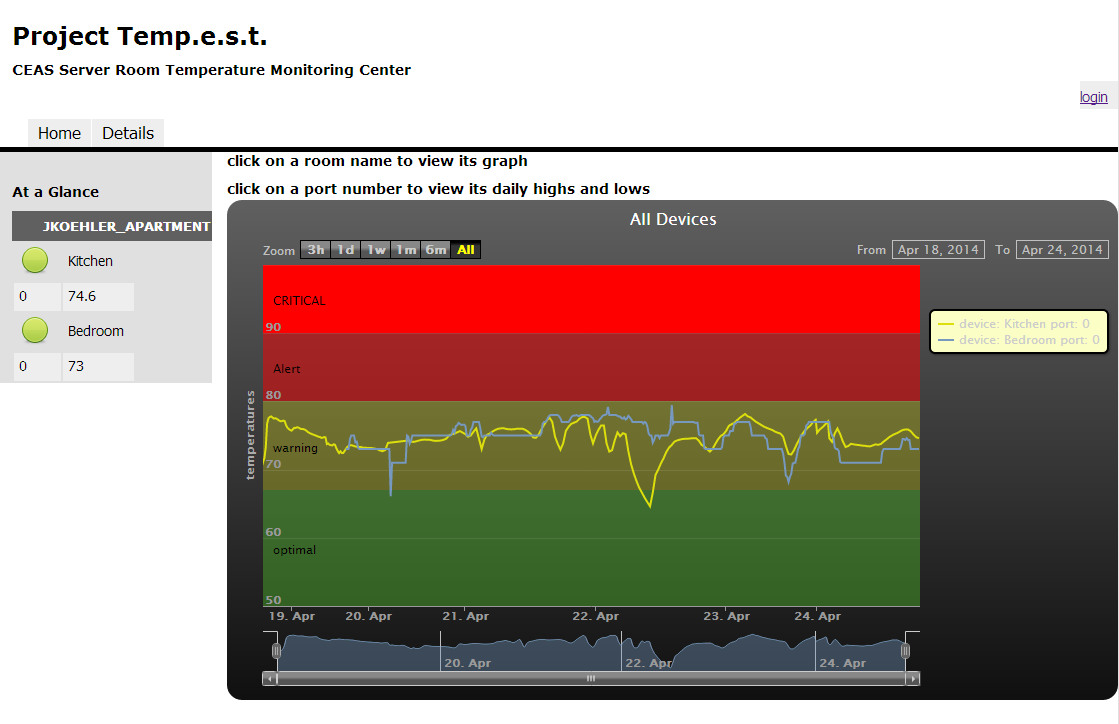
\includegraphics[scale=0.5]{Website.PNG}}
\caption{Initial View Of Site}
\end{figure}
The login process is very basic at this time but in future release will utilize stricter security, data sanitization, and input verification,
and will prevent against session hijacking, network eavesdropping, cross site scripting, and brute force attacks. 
At this time the page will simply have a “Username” and “Password” field (along with a submit button) which will have functionality
added that disables the browser from remembering or saving this information. 
Our first “alpha” release will be using a test database with test users, test usernames, test passwords, and test data, so the security
will not be an issue during this phase. When the user submits, the framework will reference the data to see if it matches what is in the database, and if it does, provide further access to the site, and if not, it will require the user to try again. 
\newline
\indent
There will be only one login page, but based on whether the user successfully authenticates as an administrator or a simple user will determine the pages and views they have access to. 
The admin will have access to the identical pages as the user, but will have an administrator functionality added to the pages, which will allow them to add new users, rooms, and devices, as well as delete or modify existing users, rooms, and devices. 
A regular user will have a list of devices, whereas an administrator will see the same list but will have a button above said list that takes them to an “add device” page.  
The list will have an “edit” and “delete” button next to each device for administrators as well. The edit and delete pages will be similar to the add page, and will be basically the same for users, devices, and rooms. 
\begin{figure}[H]
\makebox[\textwidth]{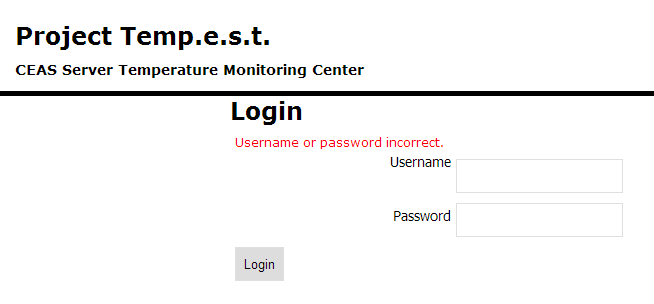
\includegraphics[scale=0.75]{LoginPage.PNG}}
\caption{Login Page}
\end{figure}
\newpage

Upon logging in as a system administrator this is what the admin will see.
This is the general hub for editing anything on the site.
From here the admin can see rooms, users, room assignments and device types easily.
The page looks just the same for a room administrator when logging into the site. 
The only difference is that the room user won't have the option to edit any rooms, devices etc.
If a non logged in user tries to access this page it will redirect them to the login page so that all admin data isn't available to the public.

\begin{figure}[H]
\makebox[\textwidth]{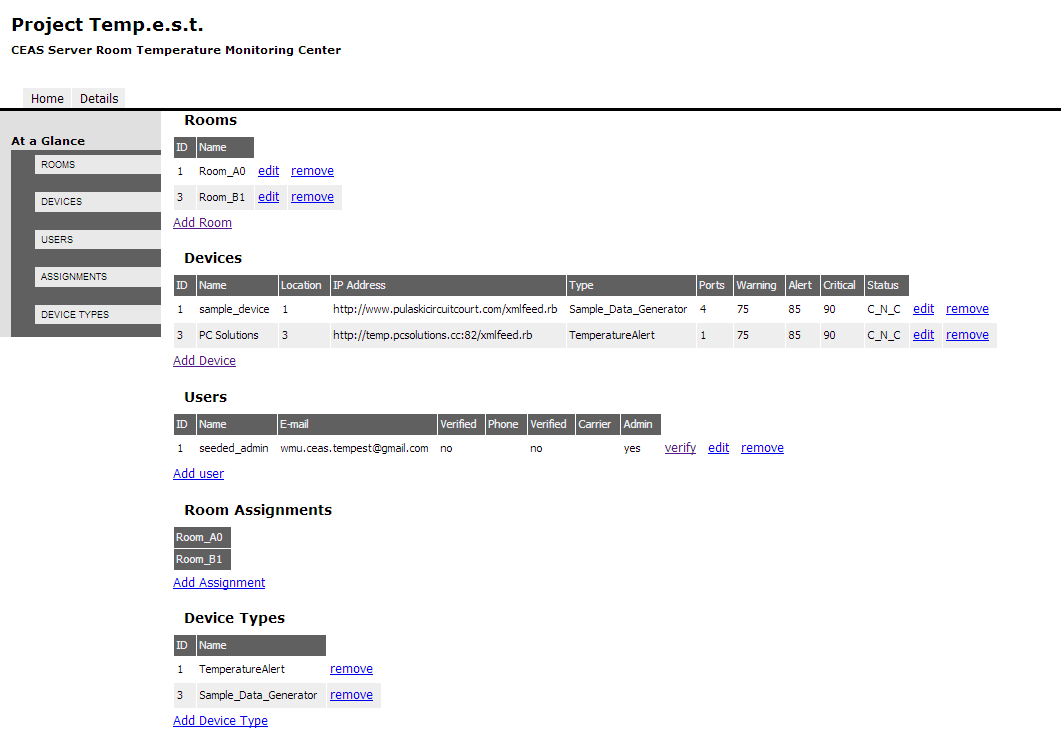
\includegraphics[scale=0.5]{AddPage.PNG}}
\caption{Add Page}
\end{figure}

The following figure is the form used when adding a new device to the network.
The IP address is a major need in this form because it tells the server where to look for the xml. 
The alert and critical thresholds are for when to warn administrators for that room.
The number of ports specifies simply the number of temperatures to expect coming from that device.

\begin{figure}[H]
\makebox[\textwidth]{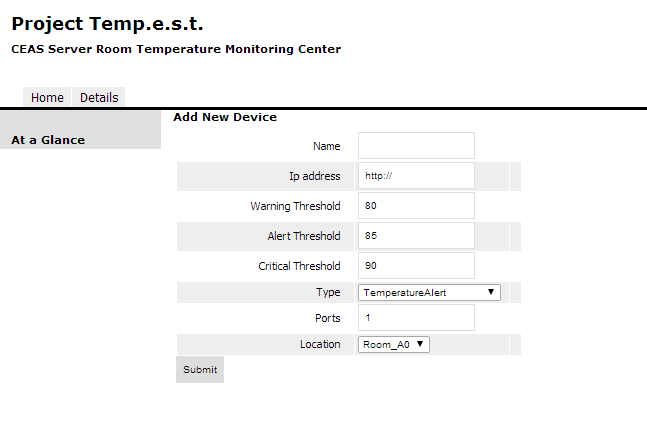
\includegraphics[scale=0.75]{AddDevice.PNG}}
\caption{Add Device To Network Page}
\end{figure}


\begin{figure}[H]
\makebox[\textwidth]{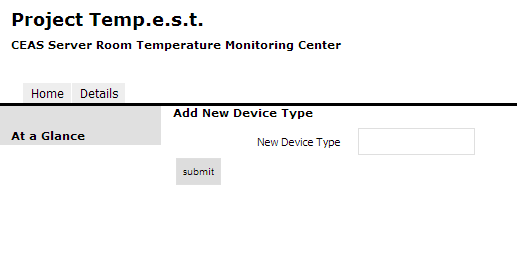
\includegraphics[scale=0.75]{AddDeviceType.PNG}}
\caption{Add Another Device Type}
\end{figure}

The following page is used to add a room to the monitoring system.
The main purpose of a room is to group sensors together and make it easier to distribute work among the administrators.

\begin{figure}[H]
\makebox[\textwidth]{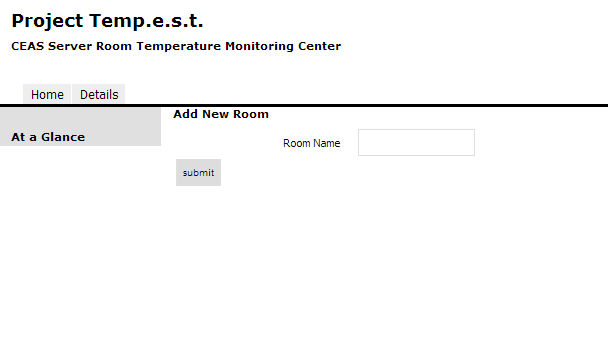
\includegraphics[scale=0.75]{AddRoom.PNG}}
\caption{Adds a Room}
\end{figure}

There are three different levels of users.
The highest level of user is the main system administrator.
This administrator is in control of the whole system. 
Their permissions include but are not limited to adding new users, adding new devices, adding new rooms etc. 
The second tier of user are the normal room administrators.
The room administrators are able see the stats of the rooms they have access and will receive alerts for those rooms.
The last layer of user is the non-registered user. 
This user can see the graph of data on the front page and login. 
It is beneficial to have it this way in case an administrator wants to quick check things and doesn't want to bother with logging in.
Below shows the form for adding a new user. The required fields are name, email, and password. 
The password does have minimal requirements for good passwords.
\begin{figure}[H]
\makebox[\textwidth]{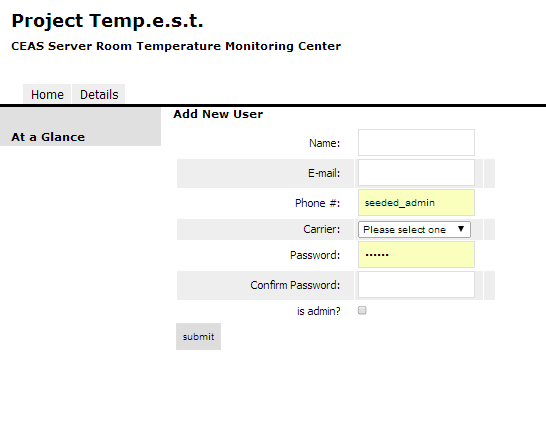
\includegraphics[scale=0.75]{AddUser.PNG}}
\caption{Page To Add Users}
\end{figure}


\begin{figure}[H]
\makebox[\textwidth]{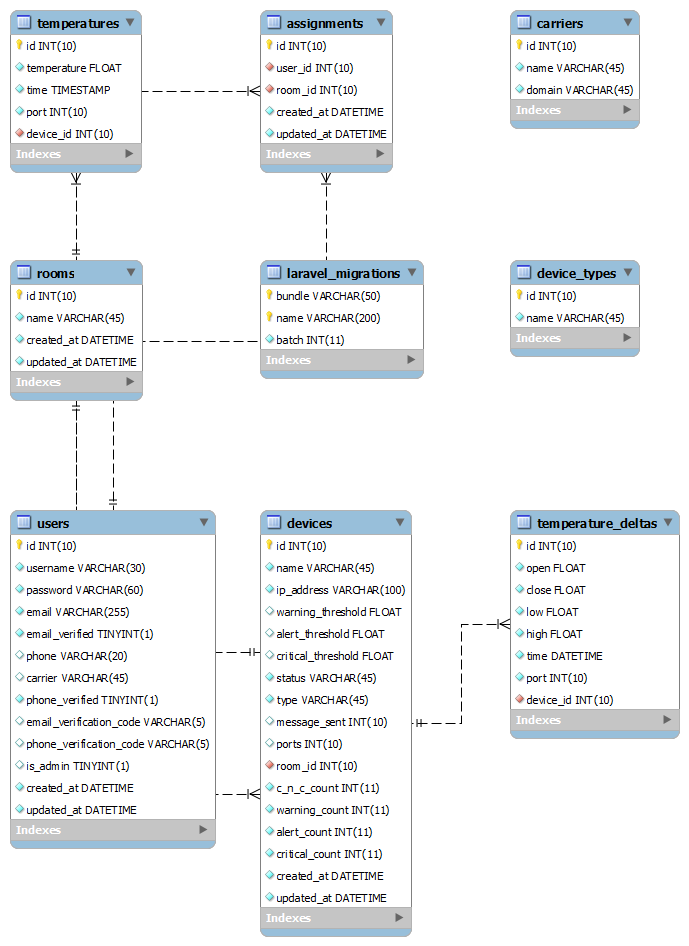
\includegraphics[scale=0.35]{ERDDiagram.png}}
\caption{Entity Relationship Diagram}
\end{figure}

\newpage
\subsection*{Design Decisions}
\addcontentsline{toc}{subsection}{Design Decisions}
\begin{itemize}
\item Raspberry Pi: We decided to use the to connect to the temperature and humidity sensor because it is cost efficient and is able to send and receive data from the monitoring server. 
Other alternatives we looked at are the Arduino and the MSP430, but we ended up deciding on the raspberry pi because there was more documentation and had all the required hardware in one bundle.
Also Raspberry Pi’s require less hardware configuration allowing a end user with less hardware skills to still be able to utilize our project.
\item Git: Team members were more familiar with the workings of Git and could be used with a GUI.
\item Sensor: For our case we will be using a humidity and temperature sensor that we found on Adafruit's website.
The sensor is called the DHT11 basic temperature-humidity sensor. 
For easy reference it is currently product number 386.
Although this sensor is cheap it has enough power to determine the temperature and humidity of a room easily.
Several limitations that the DHT11 has is it can only poll the temperature every 3-5 seconds and has a resolution of $1\,^{\circ}{\rm C}$ with an accuracy of $\pm$.$2\,^{\circ}{\rm C}$. 
Figure below is the DHT11.

\begin{figure}[H]
\makebox[\textwidth]{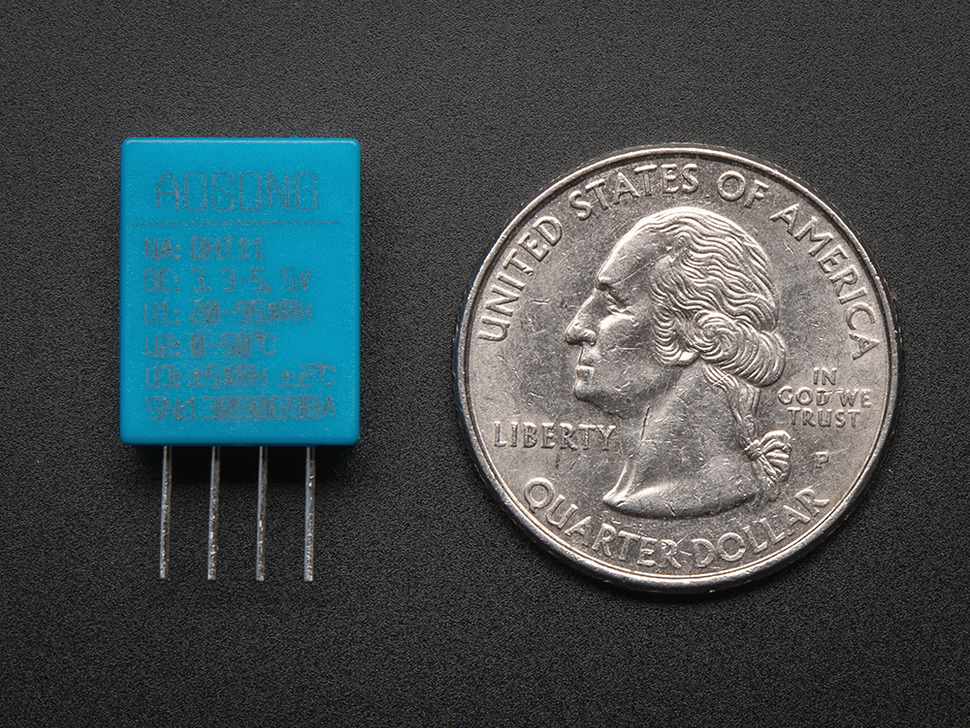
\includegraphics[scale=0.5]{tempsensor.jpg}}
\caption{Temperature Sensing DHT11 Unit.}
\end{figure}

\begin{figure}[H]
\makebox[\textwidth]{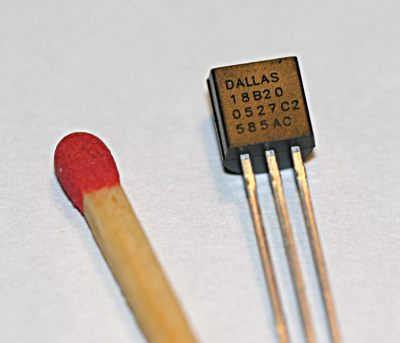
\includegraphics[scale=0.5]{ds18b20.jpg}}
\caption{A DS18B20 sensor for size comparison.}
\end{figure}


With the limitations previously mentioned, we will be exploring other sensor alternatives. There are many others that very in price, accuracy, range, and resolution, and those we have looked into are in the chart below. The sensor that the Temperature @lert device that WMU provided us uses the DS18B20 sensor, which has a comparable cost and much greater resolution. Our team is currently working on modifying an existing driver or building our own for use with our Raspberry Pi. The DS18B20 has a low cost to begin with, but can be bought in bulk for further reduced prices.  Due to their small size, it would be extremely quick and easy to bind/wrap either the DHT11, DHT22, or DS18B20 into a cable that would have an RJ-45 connector on the end, whereas it would be just as easy to have our custom 3d-printed RaspberryPi case have an RJ-45 jack so there would be no direct wiring/soldering to the RaspberryPi, and the sensors could be removed on a whim for storage, transport, or replacement should a single sensor go bad. The DHT11 and DHT22 have one great advantage over the DS18B20 in that the latter does not contain a humidity sensor, hence the smaller package.

\begin{figure}[H]
\makebox[\textwidth]{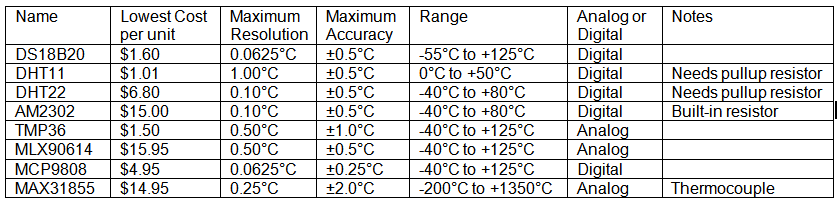
\includegraphics[scale=0.75]{sensor_comparison.jpg}}
\caption{Alternative Sensors to DHT11}
\end{figure}



\item Laravel: Although our team lacks experience with the Laravel system we decided that using the old team's code would be worth the steep learning curve of the Laravel system.
\item Cake PHP: Looking at Cake PHP we determined that though this is a very great framework the existing code should be used.
\end{itemize}
We have also decided to separate the project into 4 main functional pieces which each need their required spikes. The flow of the normal communication is as displayed as below.
\begin{figure}[H]
\makebox[\textwidth]{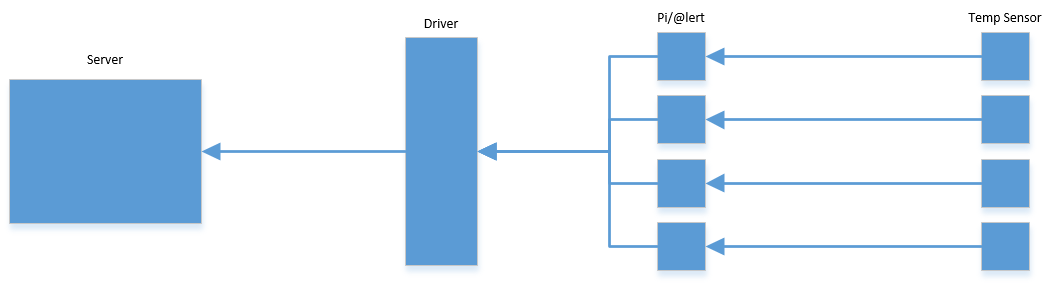
\includegraphics[scale=0.5]{DataFlowFlowChart.PNG}}
\caption{How the Data Goes Through The System}
\end{figure}
The first part in the process is getting the temperature from the device. 
For the WiFi @lert system this has been already done by the manufacture. 
As for the Pi we have a program that will read the temperature and output it to standard output.
We have two options we can either create our own custom version of the code the company supplied, or we can create a program that uses their code to get the temperature.
Both of these options are viable and both equally easy to do. 
However, both will need their respective spikes.
\newline
\indent
The next step is to create a way for the devices to communicate with the server.
Currently the @lert system does this by hosting an xml document that the server retrieves.
Our current prototype of the raspberry pi has duplicated this functionality and does require a separate parser.
The two options that we are looking at for enabling the hosting of the xml document are either apache or Nginx.
Another option is to not use a hosting program and to use a program that will give data to any requesting process.
We will have spikes for all options and determine which will be the best for the low memory that a raspberry pi has.
\newline
\indent
The third step is for the server to decode what data was received. 
This done by the parser factory PHP task.
What the parser factory does is it takes in a type and an IP address.
Then it does a switch statement based on the type and returns an object that contains the correct methods for that reader type.
For our Raspberry Pi module we will need to make an object to parse its data and an entry in the ParserFactory to detect the new object.
The object for the Raspberry Pi module will need to use the ITemperature Parser PHP interface in order to be used correctly.
In theory this can all be done using the GUI that was created by the previous team, but both the GUI and the manual method should be tried.
\newline
\indent
The final piece in the data retrieval process is the server parsing and using the data. 
If we follow the guidelines that were established by the previous groups temperature sensing unit the server should be able to treat them both the same with their respective data.
We will be using the other groups code for graphing, mygraph.js.
In this it reads in all the data for the devices. 
Our device will simply be put in with the rest of the devices and report itself with the other devices.
\newline
\indent
\newpage

\subsection*{Stories -- Requirements}
\addcontentsline{toc}{subsection}{Stories -- Requirements}
This project requires a server running Linux, and in our case we will be using Ubuntu on this system. 
The project will also require a web server that runs any 2.x version of Apache, which according to W3Techs is used by 58.70$\%$ of all websites as of March 30th, 2014.
The choice to utilize Apache 2.x-compliant technologies was made with the idea that the majority of web servers utilize this technology, so it will be accessible to the majority. 
We also require a temperature sensor of your choice.
We will be using the DHT11 and our tutorials will be using this part. 
We will be interfacing with two devices at first, beginning with the Temperature @lert WiFi edition TM-WIFI220, seen here:
\begin{figure}[H]
\makebox[\textwidth]{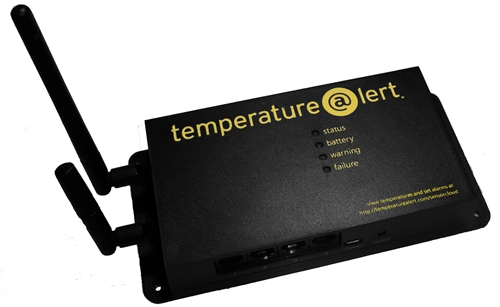
\includegraphics[scale=0.5]{AlertWiFi.PNG}}
\caption{@lert WiFi edition TM-WIFI220}
\end{figure}
 which has an initial cost of US $\$$300.00 +tax/shipping, a size footprint of H: 1.25”, W: 4.00”, L: 6.00”, an overall volume (excluding antennae) of 30 cubic inches, supports PoE, has a yearly estimated power usage of $\$$7.77 (based on 24 hour use @ $\$$0.1348 per kilowatt hour, and as is not able to be physically upgraded or added on to outside of its two available temperature and humidity sensors.
\newline
\indent
We are also designing our own sensing device that utilizes Raspberry Pi’s running Raspbian, with a generic case it would appear as the following:
\begin{figure}[H]
\makebox[\textwidth]{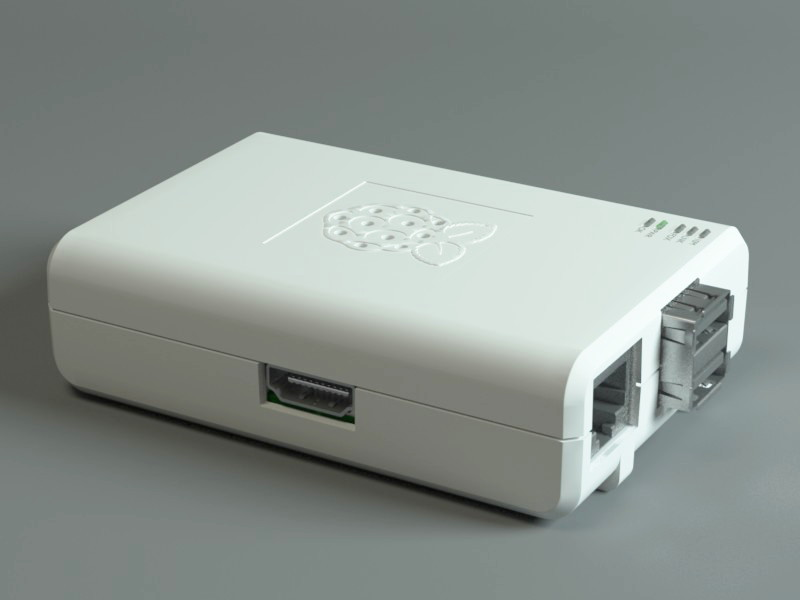
\includegraphics[scale=0.35]{Rasp.PNG}}
\caption{Example of Raspberry Pi}
\end{figure}
which has an initial cost of US $\$$61.47, a size footprint of H: 1.00”, W: 2.80”, L: 3.80”, an overall volume (excluding antennae) of 10.64 cubic inches, could potentially support Power over Ethernet (PoE), has a yearly estimated power usage of $\$$5.89 (based on 24 hour use @ $\$$0.1348 per kilowatt hour, and as is fully upgradeable in any capacity.
Some example upgrades could be light sensors (for knowing if a windowless room has its lights on or off), motion sensors (to indicate movement in the room), video/still camera (for security monitoring), or even a touch screen (for things like giving the unit the ability to edit settings without connecting to a computer, or using as an employee time clock as an example).
The possibilities are endless.
If you would like Wi-Fi connectivity for your Raspberry Pi like we are going to, we will use a wireless receiver. With the wireless functionality, this requires the unit to simply be plugged in to a power outlet as no physical network connection is required. The Wi-Fi at CEAS has extremely poor signal in places due to several factors including metal anti-theft grates that inadvertently shield them, as well as the very thick concrete walls. If the client desired, a future release of the unit could include an optional network port so that it could be wireless and wired for network connectivity redundancy in the cases that the Wi-Fi signal is poor as the unit is placed in a signal dead zone, or that the Wi-Fi goes out but the LAN would still be active.  Either way the system would alert the designated users if the units lost connectivity.
\newline
  As the Temp @lert is $\$$300 per unit, and our RaspberryPi is $\$$60, that is a cost savings of 80%.  When compared to other companies products, it is an even greater cost savings as seen here:
\begin{figure}[H]
\makebox[\textwidth]{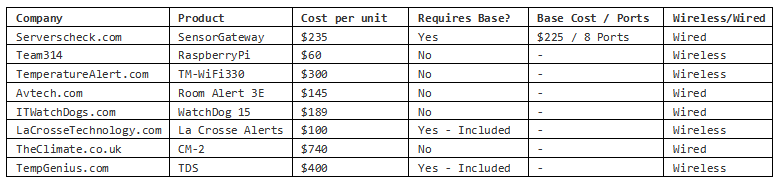
\includegraphics[scale=0.5]{product_comparison.PNG}}
\caption{A comparison of prosumer-grade sensor devices with the Team 3.14 RaspberryPi.}
\end{figure}
  Our research indicates that at a very minimum, a one-rack server room would require five sensors: one at the front-bottom of the rack (or top if it was top-cooled) to monitor the intake, one at the back top of the rack to monitor the outtake, one in the center of the room, one at the end of the room furthest from the cooling units, and one next to the cooling unit. With the current temperature sensors that WMU uses, this would be a $1500 investment, with one unit costing $300.  With our units, it would be a total cost of $300, so you could go the route of putting ten sensors in the room to cover all possible hot zones for the cost of two of the current sensors. The possibilities are endless with the reduced cost and easy availability of the units. 
\newpage


\subsection*{Stories -- Functional}
\addcontentsline{toc}{subsection}{Stories -- Functional}
\begin {itemize}
\item Use a temperature sensor to monitor the temperature of the servers room located on the CEAS campus.
\item Check the humidity of the server rooms located on the CEAS campus.
\item Graph the humidity and temperatures of the rooms.
\item Send the data to a server to be checked.
\item Use timers to make sure that communication with the servers are not lost
\item Send text messages and emails to the server administrators to alert them of loss of server connection and temperatures that are higher than the recommended level.
\item Establish permissions for the various administrators that will be monitoring the system.
\item Create documentation so that the next group of users can use the software
\end {itemize}
\newpage


\subsection*{Spikes}
\addcontentsline{toc}{subsection}{Spikes}
To do these stories we will be creating spikes to show that critical sections are actually plausible. 
After we do this we combine the spikes and add minor code to complete the system.
Some of our spikes include:
\newline
Connecting the temperature sensor:
\newline
\indent
Below is our development version of the temperature sensor setup.
\begin{figure}[H]
\makebox[\textwidth]{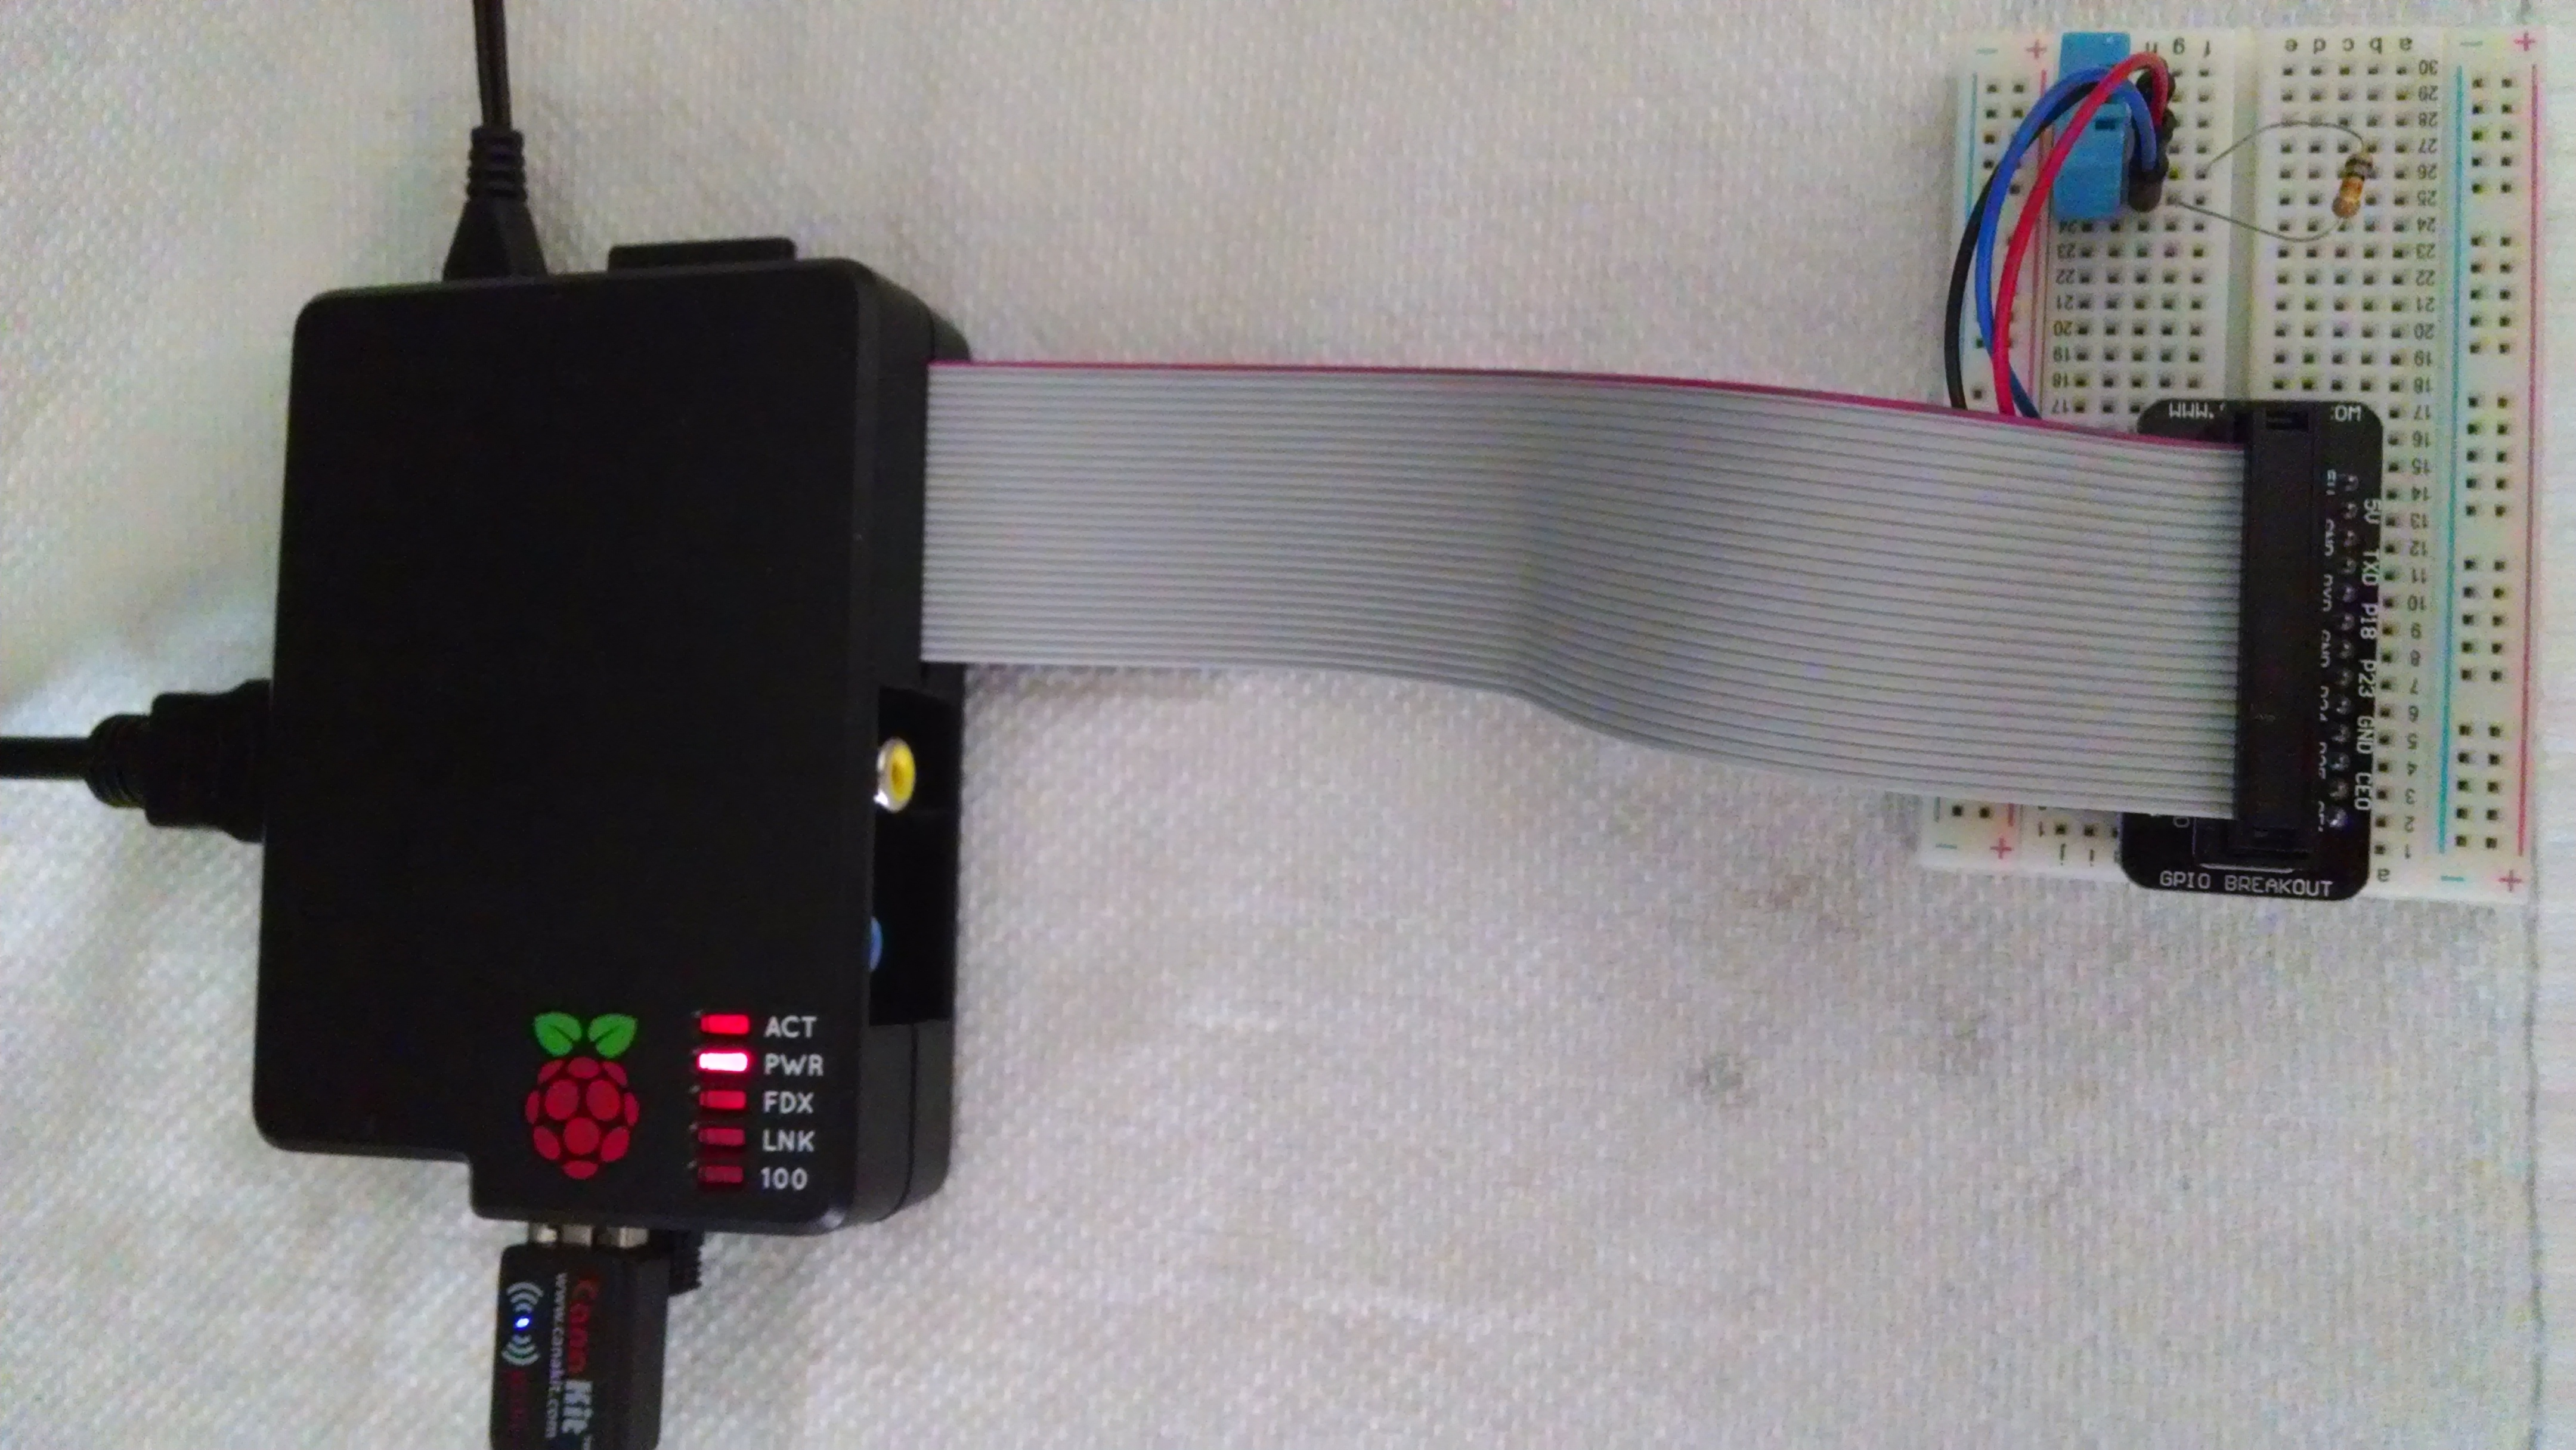
\includegraphics[scale=0.15]{fullsetup.jpg}}
\caption{Current Setup For Temperature Sensor}
\end{figure}
In the future when the project leaves the development process we would like to create a much easier way to connect the sensor and make the design more sleek.
\newline
Raspberry pi temperature retrieval code:
\newline
\indent
We have completed this spike by using code from the Adafruit website.
After examining this code we wrote our own driver for the temperature monitor that better fits our needs.
See the figure after the wireless network spike for proof of concept for getting the temperature.
\newline
Raspberry temperature to xml:
\newline
\indent
Our code for retrieving the code off of the raspberry pi immediately writes the data to the xml code that is needed to transmit the temperature over the network. 
\newline
Using Apache for hosting the xml document:
\newline
\indent
A lot of people use raspberry pi's to host websites using apache so hosting a simple XML document was very easy to accomplish by following one of the numerous guides around the internet.
\newline
Creating a driver for the Laravel code for the pi:
\newline
\indent
Based on the Laravel code that was handed down to us it was easy to create another module for the raspberry pi.
\newline
Connecting a raspberry pi to a wireless network:
\newline
\indent
Once we plugged in the wireless adapter it seemed to work right off the bat.
This was expected because it was provided by Adafruit who makes the raspberry pi's.
We also tested with other brand wireless connectors which worked equally well.
\begin{figure}[H]
\makebox[\textwidth]{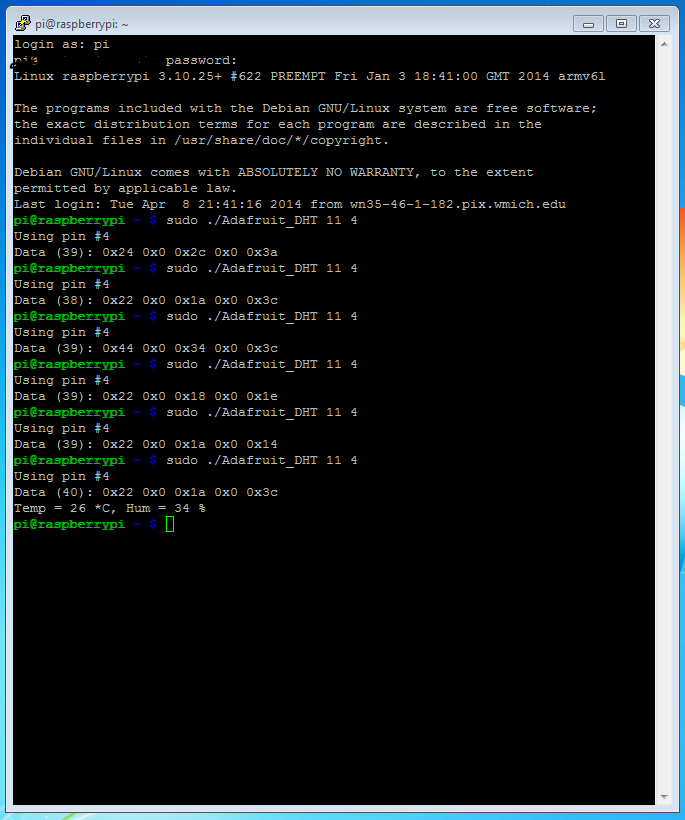
\includegraphics[scale=0.75]{ssh_to_pi.PNG}}
\caption{SSH Over Wireless Network And Sensor Data Retrieval}
\end{figure}

\begin{figure}[H]
\makebox[\textwidth]{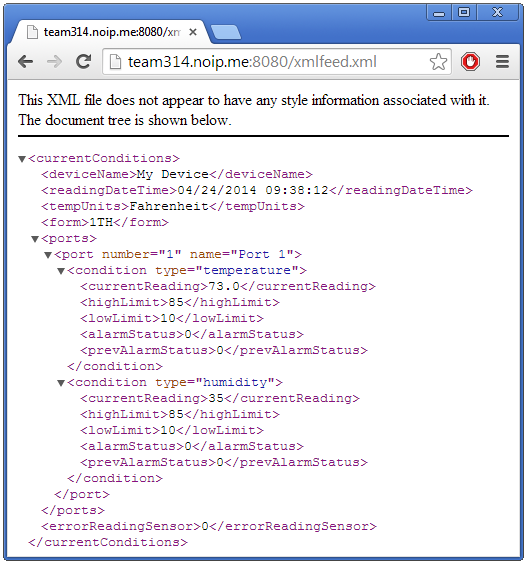
\includegraphics[scale=0.75]{raspberry_pi_xml.PNG}}
\caption{XML hosted on the RaspberryPi via Team 3.14's NoIP address.}
\end{figure}

\newpage


\subsection*{Resources}
\addcontentsline{toc}{subsection}{Resources}
\begin{itemize}
\item Raspberry Pi
\item Temperature Sensors
\item Humidity Sensors
\item Web Server
\item Soldering Equipment
\item Operating System loaded SD Cards with Raspbian
\item Power connectors for Raspberry pi
\item WiFi Connectors for Raspberry pi
\end{itemize}
\newpage
\subsection*{Feasibility}
\addcontentsline{toc}{subsection}{Feasibility}
Based the cost of the hardware and the previous source code the feasibility of this project is high with many of the features being of low to mid risk. 
We had a very informative meeting with a member from the previous senior design team where we saw how everything works and its limitations.
Based on this meeting all our goals seem very reasonable and extra features can be implemented very easily for future releases.
The biggest problem that we will encounter is the steep learning curve with the Laravel PHP package.
However, this will be overcame due to good documentation on their site and contacts with Laravel experience.
Being software oriented scientists the raspberry pi at first seemed like a daunting task. 
However, Marcel has experience with hardware and this combined with good documentation will allow for us to overcome the hardware experience issues.

\newpage
\subsection*{References}
\addcontentsline{toc}{subsection}{References}
For everything raspberry pi we use these sites
\begin{itemize}
\item http://www.raspberrypi.org/
\item http://www.raspbian.org/
\item C Programming 2nd Edition
\item http://www.adafruit.com/
\end{itemize}
For everything web server these are the sites we use
\begin{itemize}
\item http://laravel.com/docs/quick
\item http://www.w3schools.com/
\end{itemize}
\newpage
\subsection*{Glossary}
\addcontentsline{toc}{subsection}{Glossary}
\begin{description}
\item [GUI] \hfill \\
Graphical User Interface. The windows a user interacts with.
\item [MSP430] \hfill \\
A 16-bit microcontroller platform made by Texas Instruments.
\item [Raspberry Pi] \hfill \\
 A credit-card-sized single-board computer developed by the Raspberry Pi Foundation.
\item [Arduino] \hfill \\
A series of microcontrollers that are very commonly used for computer to real world communications.
\item [Raspbian] \hfill \\
 A Debian based operating system that we will use for our Raspberry Pi’s
\item [CEAS] \hfill \\
College of Engineering and Applied Sciences at Western Michigan University.
\item [PHP] \hfill \\
A recursive acronym for “PHP Hypertext Preprocessor” - the web programming language being used.
\end{description}
\newpage
\subsection*{Ownership}
\addcontentsline{toc}{subsection}{Ownership}
\begin{description}
\item [Licenses] \hfill \\
Our project will be under several licenses. PHP is a free open source software released under the PHP License.
Laravel is licensed under the MIT license and per the agreement we are “free to modify, distribute and re-publish the source code on the condition that the copyright notices are left intact”.
In the event that our project was used to generate revenue, or be sold as a standalone software package, the license permits us “to incorporate Laravel into any commercial or closed source application”.  
The GNU license and will be open source and will be hosted for all to access and modify as they desire on GitHub.
\item [Intellectual Property (IP)] \hfill \\
As this project is being developed as a Senior Design project for Western Michigan University (WMU) at the direction of Dr. John Kapenga, WMU will retain the intellectual rights to the software.
\item [Non-Disclosure Agreement (NDA)] \hfill \\
No non-disclosure agreement is being used at this time.  The project is maintained on GitHub, which is freely and openly accessible to anyone who wishes to view it, and is thus tracked by search engines such as Google, where it is able to be searched for by anyone on the planet.
\end{description}

\end{document}
